\documentclass{standalone}

\usepackage{tikz}
\usepackage{standalone}
\usetikzlibrary{calc}

\begin{document}
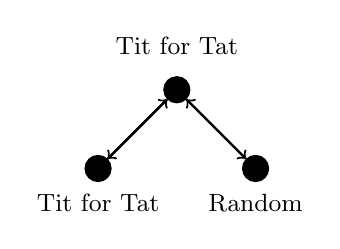
\begin{tikzpicture}

\node[draw,shape=circle,fill=black] (0) at (0, 0) [above] {};
\node[draw,shape=circle,fill=black] (1) at (2, 0) [above] {};
\node[draw,shape=circle,fill=black] (2) at (1, 1) [above] {};

\node[] (3) at (0, -0.5) [above] {\small{Tit for Tat}};
\node[] (4) at (2, -0.5) [above] {\small{Random}};
\node[] (5) at (1, 1.5) [above] {\small{Tit for Tat}};

\draw (0) edge[out=45, in=-135, ->, thick] (2);
\draw (1) edge[out=135, in=-45, ->, thick] (2);

\draw (2) edge[out=-135, in=45, ->, thick] (0);
\draw (2) edge[out=-45, in=135, ->, thick] (1);
\end{tikzpicture}


\end{document}